\documentclass[english]{article}
 
\usepackage[utf8]{inputenc}
\usepackage[T1]{fontenc}
\usepackage{babel}
\usepackage{advdate}
\usepackage{graphicx} 
\usepackage{amsmath} 
\usepackage{algorithm}
\usepackage[noend]{algpseudocode}
\usepackage{listings}
\usepackage{hyperref}

\makeatletter
\def\BState{\State\hskip-\ALG@thistlm}
\makeatother


\begin{document}
\begin{titlepage}
\SetDate[30/01/2018]
\newcommand{\HRule}{\rule{\linewidth}{0.5mm}}
\center 
\textsc{\LARGE Universite Paris Dauphine}\\[1.5cm] 
\textsc{\Large Big Data}\\[0.5cm]
\HRule \\[0.4cm] { \huge \bfseries
Single-source shortest path - Djikstra Algorithm}\\[0.4cm] \HRule \\[1.5cm]
\begin{minipage}{0.4\textwidth}
	\begin{flushleft} \large
		\emph{Students}
		\\ Elie \textsc{Abi Hanna Daher}
		\\ Bilal \textsc{El Chami}
		\\ Badr \textsc{Erraji}
	\end{flushleft}
\end{minipage}
~
\begin{minipage}{0.4\textwidth}
	\begin{flushright} \large
		\emph{Professor} 
		\\ Mr Dario  \textsc{Colazzo}
		\\  \hspace{1cm}
		\\  \hspace{1cm}
	\end{flushright}
\end{minipage}\\[2cm]
{\large \today}\\[2cm]

\includegraphics[width=8cm]{img/dauphine.png}
\vfill
\end{titlepage}
 
\tableofcontents 
\newpage

\section{Project goal}
The goal of the project is to find the shortest paths from a source node to all other nodes in the graph using the Dijkstra’s algorithm. The algorithm should be implemented in both Python-Hadoop and Spark. \\

A long side the implementation, a scalability experiments is needed to check the performance of the algorithm implemented.\\

You can find source code, data samples, documentation, etc in our repository : \href{ https://github.com/bilal-elchami/bigdata}{github.com/bilal-elchami/bigdata} .

\section{Dijkstra Algorithm}
The Dijkstra’s algorithm finds the shortest path from source to all other nodes. The djikstra algorithm is very similar to the BFS algorithm, the only difference is that the distance between neighbors isn't 1, distance can differ from a neighbor to another.\\

One of the most common and well-studied problems in graph theory is the single-source shortest path problem or Dijkstra’s algorithm, where the task is to find shortest paths from a source node to all other nodes in the graph (or alternatively, edges can be associated with costs or weights, in which case the task is to compute lowest-cost or lowest-weight paths).This algorithm is very similar to the Breadth-first search algorithm, the only difference is that the distance between neighbors isn't equal to 1 but it can differ from a neighbor to another.\\

However, this algorithm assumes sequential processing. So, the challenge was to solve this problem in parallel, and more specifically, with a MapReduce job. This section will be discussed later in the Mapper/Reducer sections of this document.

\newpage
\section{Implementation}
\subsection{Input}
\subsubsection{Data}
The map task should receive the following information
\begin{itemize}
\item node
\item distance
\item neighbors data that contains the list of neighbors with their respective distance to the node
\item path
\end{itemize}
So let's take the following example with 1 being the start node :
\begin{figure}[h]
\centering
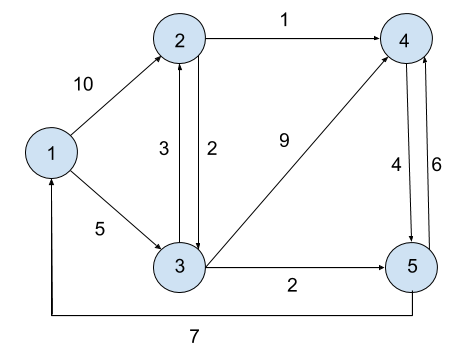
\includegraphics[width=8cm]{img/data-example.png}
\caption{Example of a graph}
\end{figure}
\\
For the first iteration, the path will be empty. So input data will look like this :
\begin{itemize}
\item 1 0 2,10:3,5:
\item 2 999 3,2:4,1:
\item 3 999 2,3:4,9:5,2: 
\item 4 999 5,4:
\item 5 999 1,7:4,6:
\end{itemize}
So as you can see, the start node has a distance of 0, and all other nodes have a distance of 999 which represent an infinite number. The neighbor list contains each neighbor node with their respective distance, the neighbors and the distance are separated by a "," and neighbors are separated by ":".

\subsubsection{Prepare}
Technically, the format we set for the data is very hard to implement to a large graph. Usually the graph is represented by the distance between nodes. So for the graph provided in the previous page, the input data will look like this 
\begin{itemize}
\item 1 2 10
\item 1 3 5
\item 2 3 2
\item 2 4 1
\item 3 2 3
\item 3 4 9
\item 3 5 2
\item 4 5 4
\item 5 1 7
\item 5 4 6
\end{itemize}
We created a job MapReduce - called prepare that will format the usual format of a graph to the format we are asking for.\\

The prepare algorithm will take in consideration the nodes that dont connect to another node but is a neighbor for another node.

\newpage
\subsection{Mapper}
A map task receive (K,V)
\begin{itemize}
\item Key : node
\item Value : distance, neighbors data, path
\end{itemize}
In the first iteration, the path will be empty. \\
The map task will : 
\begin{enumerate}
\item emit the node with his information (distance, neighbors data and path)
\item  $\forall$ neighbor $\in$ neighbors, it will emit 
	\begin{itemize}
	\item Key : neighbor
	\item Value : (node distance + distance of node to the neighbor , node path + neighbor).
	\end{itemize}
\end{enumerate}

The pseudo code of the mapper is as follow : 
\begin{algorithm}[h]
\caption{Mapper}\label{mapper}
\begin{algorithmic}[1]
\Procedure{Map \emph{(node, (distance, neighbors, path))} }{}
\State \textbf{Emit} \emph{(node, (distance, neighbors, path))}
\State \textbf{for all} \emph{ neighbor $ \in$ neighbors } \textbf{do}
\State $\textit{ dist} \gets \textit{distance} + \textit{neighbor.distance} $
\State $ \textit{ p} \gets \textit{path} + \textit{neighbor.id} $
\State \textbf{ Emit} \emph{(neighbor.id, (dist, p))}
\EndProcedure
\end{algorithmic}
\end{algorithm}

\newpage
\subsection{Reducer}
The reducer will gather the possible distance for each node. it selects the minimum distance and gives its associated path .\\

The reducer task will iterate through the nodes generated from the mapper task and for each node it will :
\begin{enumerate}
\item identify if the node contain the data structure or just a distance
\item identify the minimum distance of the node
\item Emit the minimum distance and the graph structure with the path
\end{enumerate}

The pseudo code of the reducer is as follow : 
\begin{algorithm}[h]
\caption{Reducer}\label{reducer}
\begin{algorithmic}[1]
\Procedure{Reducer \emph{(node, [(distance, neighbors, path), (distance, path),...])} }{}
\State $ d_{min} \gets \infty $
\State $ nodePath \gets \emptyset $
\State $  graph  \gets \emptyset $ \\

\State $for \quad v \in values $ \\

\If{isNode(v)}
	\State $ d_{min} \gets  v.distance  $
	\State $ nodePath \gets v.path $
	\State $ graph \gets  v.neighbors $
\Else{}
	\If{$ v.distanced_{min} \leq d_{min} $}
		\State $ d_{min} \gets  v.distance $
		\State $ nodePath \gets v.path $
	\EndIf
\EndIf

\State \textbf{ Emit} \emph{(node, ($d_{min}, graph, nodePath$))}

\EndProcedure
\end{algorithmic}
\end{algorithm}

\newpage
\subsection{Job Chaining}
Since Dijkstra algorithm is iterative and we were using Python streaming in for the project, we needed to execute several MapReduce steps with overall job scenarios, which means the last reduce output will be used as input for the next map job.\\

Map1 $\rightarrow$ Reduce1 $\rightarrow$ Map2 $\rightarrow$ Reduce2 $\rightarrow$ Map3... \\


 the simplest way to achieve it was by creating a shell script, that automates what we were doing manually.\\

The script launches the Hadoop Streaming job, merges the output parts into one file and then moves it into the data directory so it can be used as input for the next job.\\

It’s not the optimal solution but it can do the job in an “acceptable” amount of time.\\

In spark, we didn't face any problem with the iteration, since we can do it with a simple while or for loop.\\

The Job Chain script is available on another github repository : \\
\href{https://github.com/bilal-elchami/hadoop_streaming_job_chaining}{$https://github.com/bilal-elchami/hadoop\_streaming\_job\_chaining$}.

\newpage
\section{Code description} 
Source code can be found in the appendices or in the github repository.\\
\subsection{Hadoop}
The MapReduce python code was a straight forward implementation of the pseudo code elaborated above. We didn't find any difficulties implementing the algorithm. 
\subsection{Spark}
The conception of the script has been adapted according to the Hadoop streaming job. \\
The loop breaking condition is identified with the help of an accumulator that breaks the loop when the distances at every node no longer change at the next frontier.\\

\begin{figure}[h]
\centering
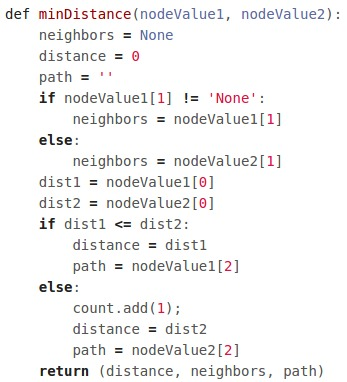
\includegraphics[width=8cm]{img/min-distance.jpeg}
\caption{Incrementation of the accumulator in min distance function}
\end{figure}

\begin{figure}[h]
\centering
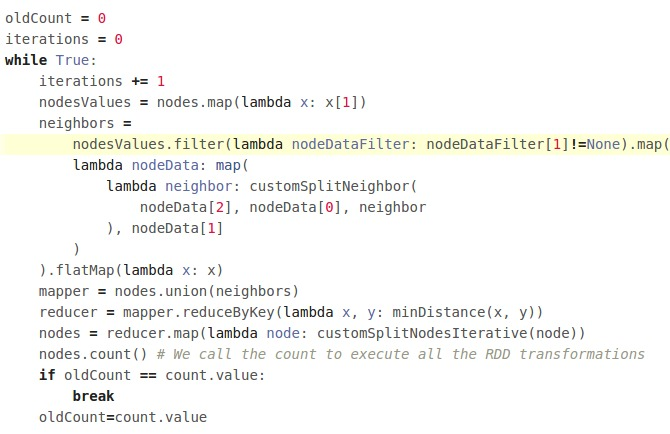
\includegraphics[width=12cm]{img/loop.jpeg}
\caption{Breaking condition to terminate the algorithm}
\end{figure}

The accumulator was used as a flag representing if the distance of a node was changed in the “minDistance(nodeValue1, nodeValue2)” function as you can see in the above code

\newpage
\section{Results}

You can check the execution commands in the README file in the repository.\\
\subsection{Hadoop}
When we pass the above graph as input to the Hadoop streaming MapReduce, the output file will contain the following data\\
$ $\\
$ 1\quad  0\quad 2,10:3,5:\quad 1$\\
$ 2 \quad 8\quad 3,2:4,1: \quad1\rightarrow3\rightarrow2$\\	
$ 3\quad  5 \quad2,3:4,9:5,2: \quad1\rightarrow3$\\	
$ 4 \quad 9 \quad5,4: \quad 1\rightarrow3\rightarrow2\rightarrow4$\\	
$ 5 \quad 7 \quad1,7:4,6: \quad1\rightarrow3\rightarrow5$\\
$ $\\
And each element in each line represents:
\begin{itemize}
\item the current’s node id
\item the calculated distance from the “Start Node” to the “Current Node”
\item the neighbors of the “Current Node” with its distance
\item the shortest path found from the “Start Node” to the “Current Node”
\end{itemize}

\subsection{Spark}
The following output represents the spark calculation results. It is the same as the Hadoop output but without the unnecessary neighbors data.\\
\begin{figure}[h]
\centering
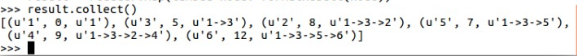
\includegraphics[width=11cm]{img/spark.png}
\caption{Example of a graph}
\end{figure}

\section{Scalability experiments}
\subsection{Data}
We used the Facebook data, that consists of friend lists from Facebook. Facebook data has been anonymized by replacing the id of the facebook of each user with a new value.\\
The graph contains $4039$ nodes and $88234$ edges. \\

The facebook data was downloaded from the Stanford's website :\\  \href{https://snap.stanford.edu/data/egonets-Facebook.html}{https://snap.stanford.edu/data/egonets-Facebook.html}.\\

We created a Map job that adds a random distance (between 1 and 10) for each intersection. The created job is a python script, and can be found under the following folder python/add-distance-graph.py in the repository. \\

After adding random distances, another map job was executed with the aim to format the data and make it compatible with our MapReduce input (check section 3.1.2).
 
\subsection{Environment}
We did the experiment on the Dauphine Cluster by using 10 cores for Spark, and 10 reducers for Hadoop Python Streaming.

\subsection{Hadoop}
The facebook data were executed 100 times on Hadoop Streaming with the help of the Job Chain Script. Each iteration took about $7.281$ seconds. The time is acceptable for the following data, but will evantually increase for bigger graphs.\\

\newpage
\subsection{Spark}
In Spark, the iteration took much more longer than Hadoop.
We faced some scalability issues with bigger graph structures. Those issues can be spotted in the formatting data section which was implemented from a more readable structure. We identified the code that was causing the latency in the execution :\\

\begin{figure}[h]
\centering
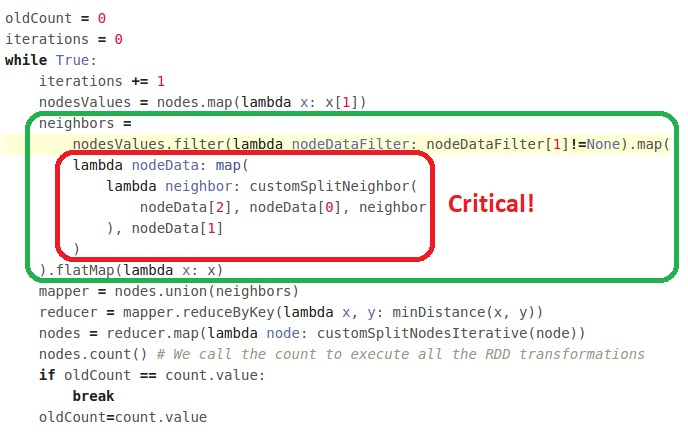
\includegraphics[width=11cm]{img/critical.jpeg}
\caption{Critical code that can be optimized}
\end{figure}

Unfortunately, it’s not the most optimized way to implement the Dijkstra’s algorithm.


\newpage
\begin{thebibliography}{9}
\bibitem{cloud-computing-lecture} \textit{Cloud Computing Lecture 4 - Graph Algorithms with MapReduce}. Jimmy Lin, The iSchool, University of Maryland, February 6, 2008.
\bibitem{github-repo} \textit{Hadoop code from github}. \href{https://github.com/Troll-Mcloving/SistemasDistribuidosAvroHadoop}{https://github.com/Troll-Mcloving/SistemasDistribuidosAvroHadoop}
\bibitem{wikipedia} \textit{Djikstra Algorithm - wikipedia page}
\end{thebibliography}
\newpage
\appendix
\section{Hadoop - Mapper python code}
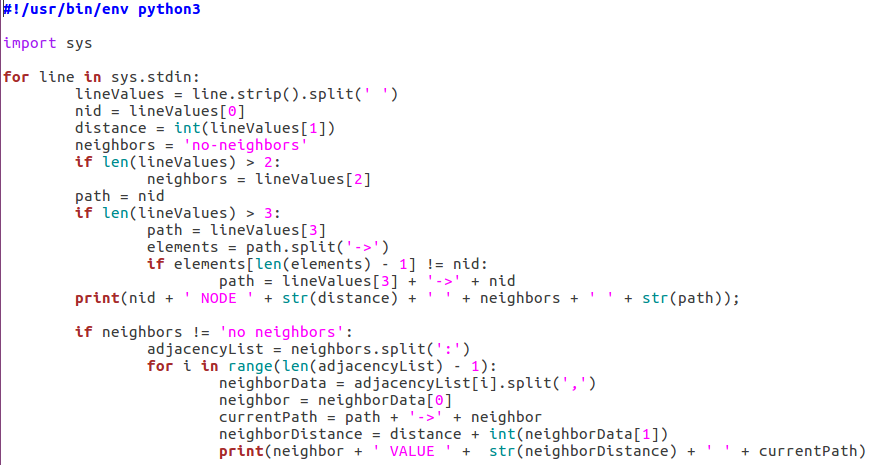
\includegraphics[scale=0.7]{img/hadoop-mapper.png}
\newpage
\section{Hadoop - Reducer python code}
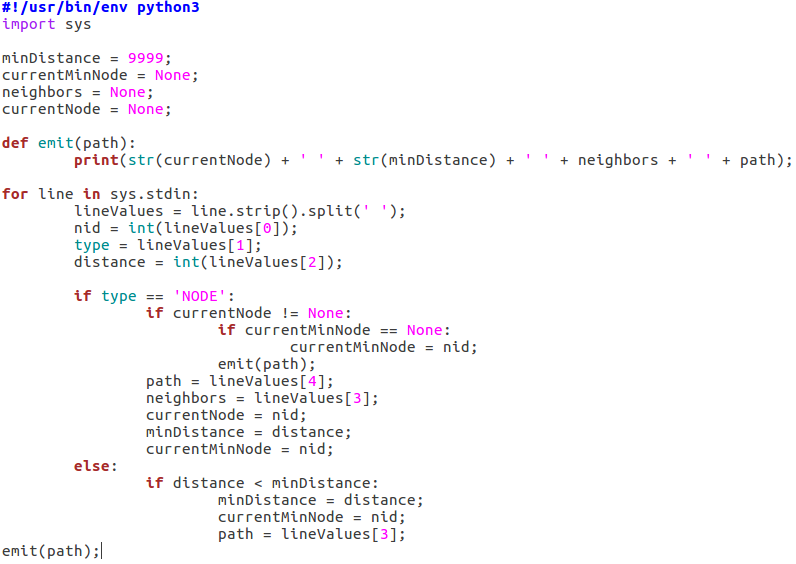
\includegraphics[scale=0.7]{img/hadoop-reducer.png}
\newpage
\section{Spark code}
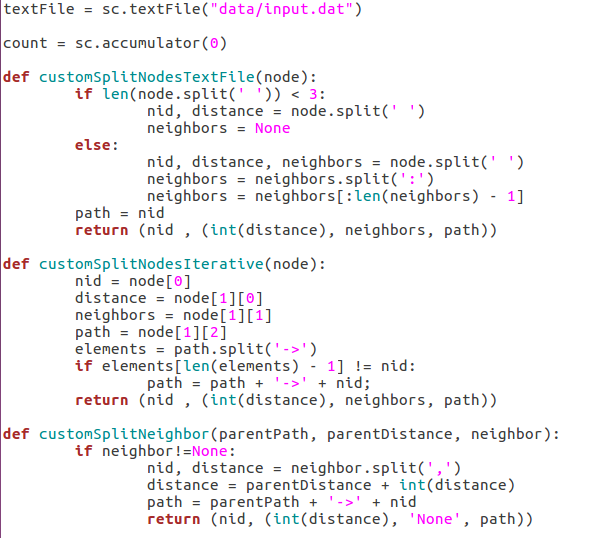
\includegraphics[scale=0.7]{img/spark-code-1.png}
$ $\\
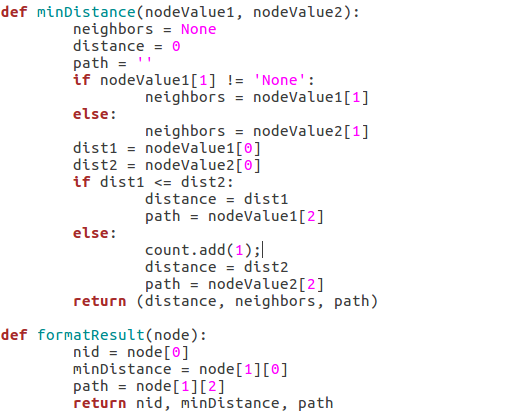
\includegraphics[scale=0.7]{img/spark-code-2.png}
$ $\\
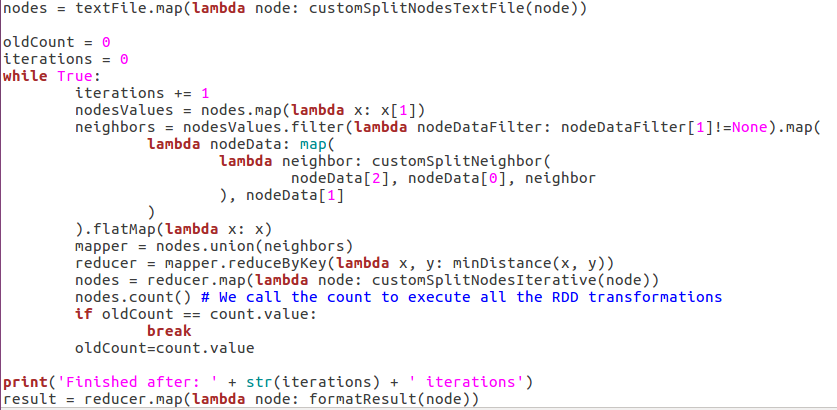
\includegraphics[scale=0.7]{img/spark-code-3.png}
\section{Prepare python code}
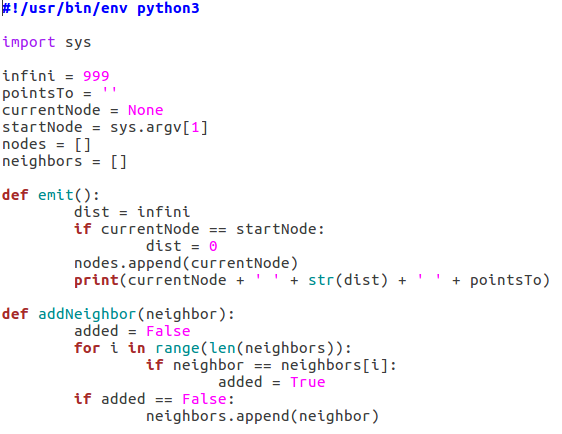
\includegraphics[scale=0.7]{img/hadoop-prepare-1.png}
$ $\\
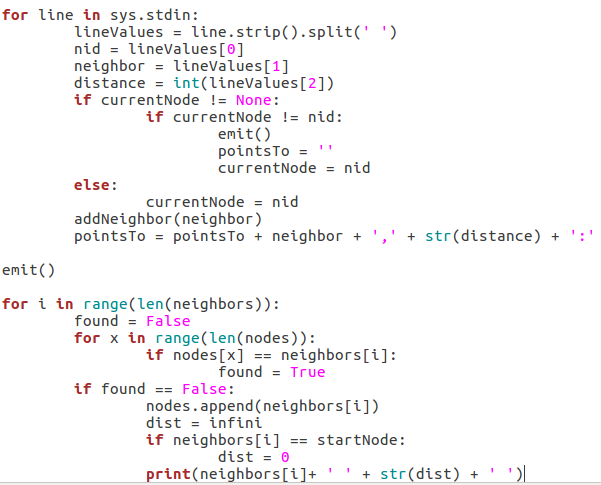
\includegraphics[scale=0.7]{img/hadoop-prepare-2.png}
\section{Add distance to graph - python code}
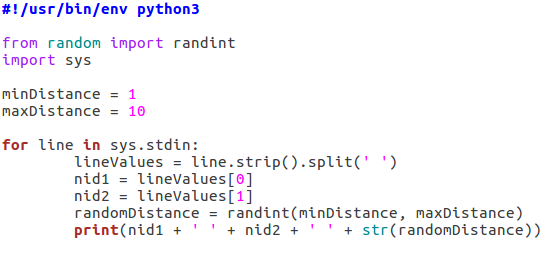
\includegraphics[scale=0.7]{img/hadoop-add-distance-graph.png}


\end{document}